\documentclass[12pt,titlepage]{article}
\usepackage{tabularx}
\usepackage{graphicx}
\usepackage{courier}
\usepackage[utf8]{inputenc}
\usepackage[T1]{fontenc}
\usepackage[english]{babel}
\usepackage{hyphenat}
\selectlanguage{english}
\usepackage{pslatex}
\usepackage{ulem}
\usepackage{url}
\usepackage{here}
\usepackage{ltablex}
\usepackage{placeins}
\keepXColumns
\makeindex
\usepackage[pdftitle={PRESCRIPTIONS MANAGEMENT SYSTEM},%
           pdfstartview={FitH}, pdftex, colorlinks=false,%
           pdfpagelabels=false, bookmarks={true}]{hyperref}
\begin{document}
\pagestyle{empty}
\begin{titlepage}
\vspace*{\fill}
\begin{center}
\begin{picture}(300,510)
 \put( 10,520){\makebox(0,0)[l]{\large \textsc{Faculty of Fundamental Problems of Technology}}}
 \put( 10,500){\makebox(0,0)[l]{\large \textsc{Wrocław University of Technology}}}
 \put( 0,290){\makebox(0,0)[l]{\Huge  \textsc{Prescription management system}}}
 \put( 70,260){\makebox(0,0)[l]{\Huge  \textsc{The patient module}}} 
 \put(70,190){\makebox(0,0)[l]{\large \textsc{Z. Dobosiewicz \& M. Niemczyk}}}
 \put(40,170){\makebox(0,0)[l]{\large \textsc{P. Nużka \& B. Paciorek \& B. Piwowarski }}} 
 \put(100,-80){\makebox(0,0)[bl]{\large \bf \textsc{Wrocław 2014}}}
\end{picture}
\end{center}
\vspace*{\fill}
\end{titlepage}
\tableofcontents
\newpage
\pagestyle{headings}
\section{\textsc{Current situation}}
The main element of the currently used system is a paper prescription. 
It contains all information required to buy specific medicines, e.g.:
\begin{itemize}
\item prescription's creation date
\item patient's personal data:
\begin{itemize}
\item name and surname 
\item address
\item PESEL
\end{itemize}
\item number of the prescription, specific for each doctor
\item list of medicines with level of refund, 
signature and stamp of the doctor
\end{itemize}
The patient, who was given the prescription by the doctor, goes to the pharmacy to buy the medicines. 
He gives his prescription to a pharmacist and says which of the medicines from the list he wants to buy.
The pharmacist checks if the medicines are available and if yes, he sells them. 
Next, he takes the prescription and makes a signature next to the each of the medicine he sold. 
He also inputs to the software installed on computers in the pharmacy, which of the medicine was sold, for who, who gave the prescription and what are the costs of the refund.
\\

A report, including detailed information about each prescription sold in the pharmacy, is generated each month. 
This report is sent to the NFZ central database. 
NFZ refunds the costs of the medicines based on this report. 
Each prescription has to be kept in the pharmacy for at least five years, and should be ready for controls made by NFZ representatives.

\newpage

\section{\textsc{Patient's module}}
\subsection{\textsc{Module description}}
The prescription system from the patient point of view is based on smart cards. 
Each patient has a unique card with ID and a pair of cryptographic keys used to create a signature. 
The system could be easily combined with electronic IDs, when they become available in Poland.
\\

The benefit of our system is that the patient could get the prescription without leaving home. 
He could request medicines by calling the doctor, who would prescribe them and make available on patient's account. 
In order to decrease the refund fraud problem, the patient has to realize the prescription in pharmacy by himself. 
If he is unable to realize it, he would be able to transfer it onto another person's account. 
Realization of a transferred prescription would only be possible for the person designed by the patient. 
However, if the patient would like to change the designed person or make the prescription again available for him to realize, he would be able to cancel the transfer.
\\

Both the patient and the doctor (with patient's permission) are able to browse all of the patient's previous prescriptions. 
It could be helpful to reduce possibility of interactions between drugs prescribed by different specialists. 
Also, doctors would not be able to abuse this functionality, because it would require the patient to insert his smart card into the terminal in doctor's office.
\\

Patient is able to browse the list of medicines, doctors and pharmacies. 
Thanks to this, he could easily check the leaflet of the medicine, find the phone number to the doctor or check the opening hours of the pharmacy.

\subsection{\textsc{Goals of the patient module}}
\begin{itemize}
\item Protection from the refund fraud problem
\item Possibility to get prescriptions without leaving home
\item Functionality of transferring prescription to another person's account
\item Availability of prescription history for a doctor
\item Possibility to browse the list of medicines, doctors and pharmacies
\end{itemize}

\newpage

\section{\textsc{Threats and inconveniences}}
The way prescriptions are currently processed is vulnerable to many threats, and brings many inconveniences. 
The most important ones are listed below.

\begin{tabularx}{\textwidth}{ |p{2.5cm}|X| }
	\hline
	\textbf{Party} &  \textbf{Threats and Inconveniences}\\
	\hline	
patient & \begin{itemize}
\item the patient can lose the prescription and he cannot buy the medicines, even if they are lifesaving, he has to go to the doctor again and ask for the new prescription
\item the patient can lose his prescription, then, the person who found this prescription can buy this medicines; what is more, this person can get to know, who takes which medicines and in this way, he can get to know, what is wrong with the person described on the prescription
\end{itemize} \\
\hline
	
NFZ & \begin{itemize}
\item significant amount of money is being defrauded from NZF, because the current system does not verify if the patient himself has bought the medicine or the pharmacists has made a false call for the medicine having some patient's prescription, prepared by the doctor (who is also a part of the defraudation scheme)
\end{itemize} \\
\hline

system & \begin{itemize}
\item the patient can try to copy the prescription and try to buy the medicines few times in different pharmacies
\item the patient can claim that he has lost his prescription and ask the doctor to give him another one, then, he can buy the medicines twice instead of once
\end{itemize} \\
\hline
\end{tabularx}

\subsection{\textsc{Protection methods}}
\subsubsection{\textsc{Smart Card}}
The main reason we decided to use smart cards is that smart card solutions, which employ two factor authentication, i.e. "something you have and something you know", provide a high security level which is crucial for the prescription system sensitive data.
\\

All of the system's users will be given personalized smart cards which will store their identification data: names, surnames, PESEL and digital certificates. 
Each card would have PIN number associated with it, that will be used to initialize authentication process.
\\

To improve the security level of the system, the data stored on smart cards should be encrypted. 
Users' private keys need to be stored in a secure memory which cannot be directly read out.
\\

In case of loosing a smart card, the user should perform a standardized revocation procedure, i.e. he should block a card in the assigned institution. 
The user should enroll for a new card afterwards

\subsubsection{\textsc{Certificates}}
Each user has his digital certificate on his smart card. 
All of the user's certificates must be given by a defined certification authority and regularly updated.
\\

The certificate's validity should be checked at each use of the user's smart card.
The validity check is performed in the database module.

\newpage

\section{\textsc{System architecture}}
The patient's module architecture consists of the following elements:
\begin{itemize}
\item smart card with personal certificate and secure key storage, used for the authentication and signing
\item patient's application, providing all of the functionalities required by patient's module:
\begin{itemize}
\item provides user-friendly interface
\item is connected with patient's card and the database
\item establishes two way SSL connection	
\end{itemize}
\item database is a central element of the whole system; stores the data and handles all the necessary database I/O functions; the database is described in greater detail in Database \& Server Documentation'
\end{itemize}

\newpage

\section{\textsc{Use Cases}}
Patients have access to the system by dedicated patient's application. 
Each patient is given unique, personal smart card that is being used for authentication.
\\
\\
\begin{figure}
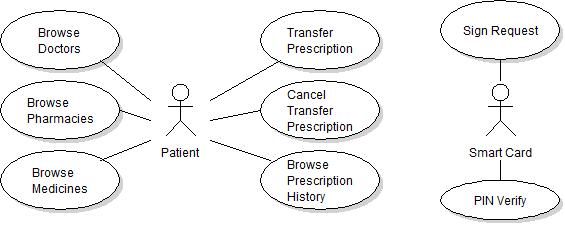
\includegraphics[width=\linewidth]{useCaseDiagram}
\caption{Use cases}
\end{figure}
\\
\\
\subsection{\textsc{Use cases for patient's application}}
The patient's application is a graphical interface to the patient's module. 
It includes six use cases that are available for the patient:
\begin{description}
\item[browse medicines] \hfill \\
The patient is able to browse all medicines available in the database. 
There is a leaflet attached to each medicine's description, that contains at least dosage and contraindications.
\item[browse pharmacies] \hfill \\
The patient is able to browse all pharmacies available in the database. 
Each pharmacy has its address and opening hours listed for patient's convenience.
\item[browse doctors] \hfill \\
The patient is able to browse all doctors available in the database. 
He can find phone number and office address for each doctor.
\item[browse prescription history] \hfill \\
The patient can browse all of his prescriptions, differentiated on active and already realized.
\item[transfer prescription] \hfill \\
If the patient cannot realize prescription, he is able to transfer his prescription buying rights to somebody else.
\item[cancel prescription transfer] \hfill \\
The patient can cancel transfer of prescription and realize it by himself or transfer it again.
\end{description}
\subsection{\textsc{Smart card use cases}}
The smart card, introduced into the system for security reasons, includes two use cases.
\begin{description}
\item[sign message] \hfill \\
The smart card signs a message produced by patient's application. 
The signature would be used in calls to database procedures.
\item[verify PIN] \hfill \\
The smart card verifies PIN, that the patient has entered, in order to access any functionalities of the system.
\end{description}
\subsection{\textsc{Flow chart for transfer prescription use case}}
To transfer the prescription user has to enter correct PIN. 
Application establish connection with database and retrieve the list of prescription available to transfer. 
The list contains only prescriptions which can be transferred by the patient. 
Then the patient is able to select prescription to transfer from the list and enter the new owner's ID. 
After the patient's confirm transfer, application create and send request to the database. 
If the signature under the request concatenated with nonce is valid and request contains required data database transfers the prescription to the new owner.

\begin{figure}
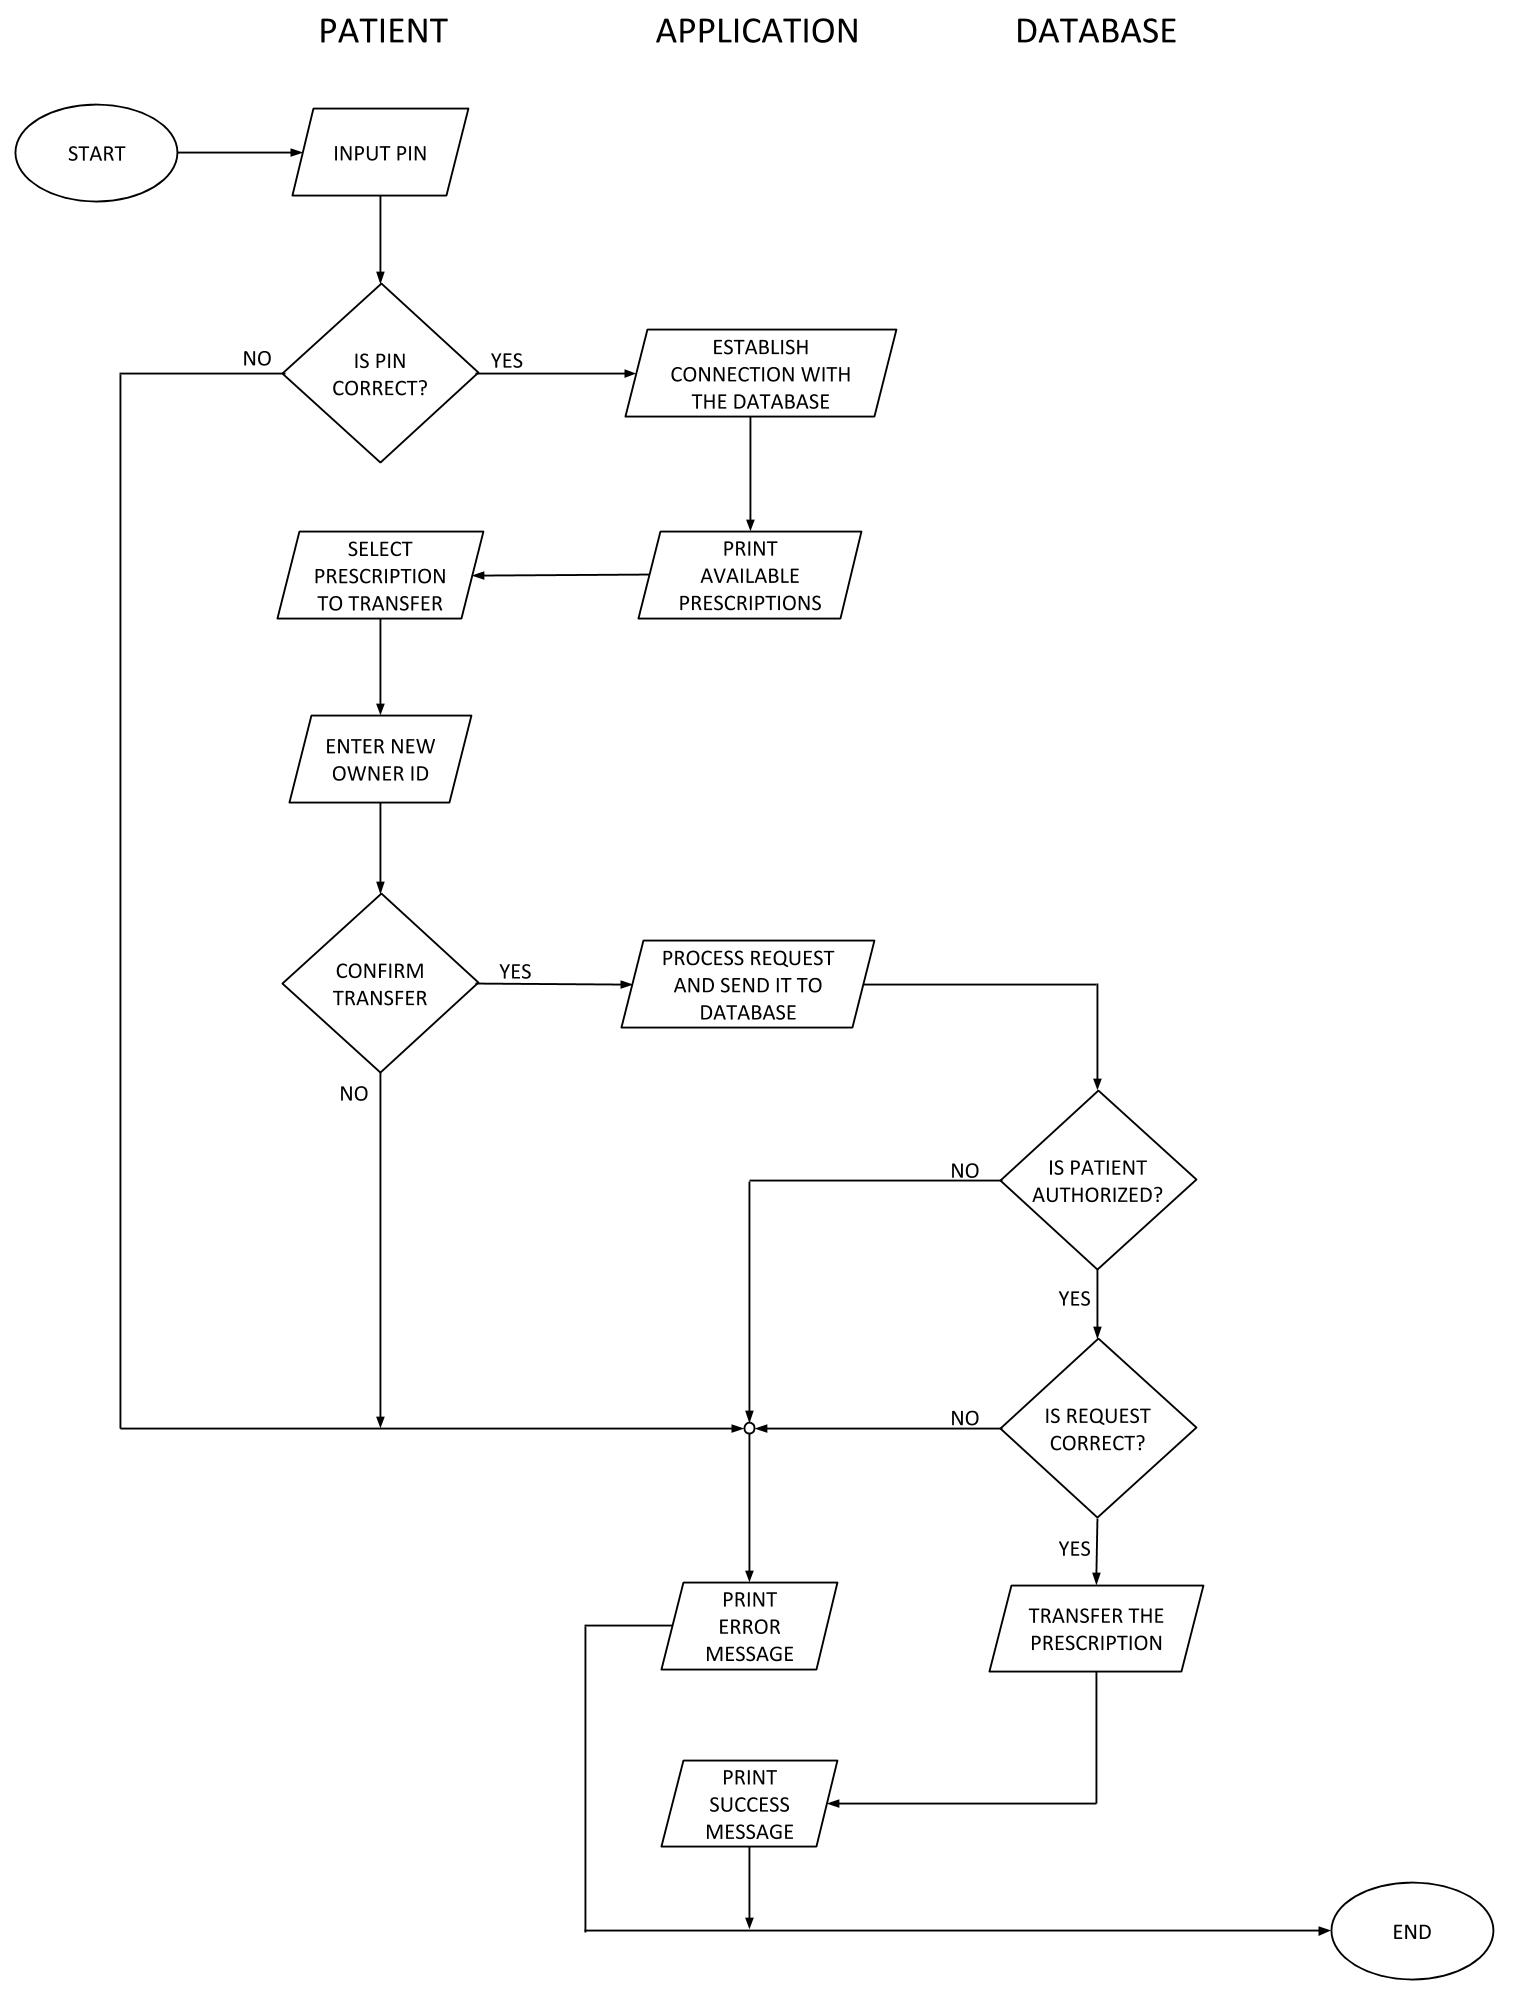
\includegraphics[width=\linewidth]{transferPrescriptionFlowChart}
\caption{Transfer prescription flow chart}
\end{figure}


\newpage


\section{\textsc{Functionalities of application}}

The application implements following functions:
\begin{itemize}
\item \texttt{browse\_medicines}
\item \texttt{browse\_pharmacies}
\item \texttt{browse\_doctors}
\item \texttt{browse\_prescription\_history}
\item \texttt{transfer\_prescription}
\item \texttt{cancel\_prescription\_transfer}
\end{itemize}
They are discussed in greater detail below.

\subsection{\textsc{Browse medicines}}

\begin{tabularx}{\textwidth}{ |p{2.5cm}|X| }
	\hline
	 &  \texttt{browse\_medicines}\\
\hline	
argumets & 
\begin{itemize}
\item \texttt{name}
\item \texttt{type}
\end{itemize} \\
\hline
description & The patient is able to browse all medicines available in database.\\
\hline
action & After entering name of medicine, function is querying database for results.\\
\hline
display &
\begin{itemize}
\item \texttt{name}
\item \texttt{prescription requirement}
\item \texttt{patient information leaflet}
\end{itemize}\\
\hline
\end{tabularx}

\subsection{\textsc{Browse pharmacies}}

\begin{tabularx}{\textwidth}{ |p{2.5cm}|X| }
	\hline
	 &  \texttt{browse\_pharmacies}\\
\hline	
argumets & 
\begin{itemize}
\item \texttt{name}
\item \texttt{address}
\end{itemize} \\
\hline
description & The patient is able to browse all pharmacies available in database.\\
\hline
action & After entering name or address of pharmacy, function is querying database for results.\\
\hline
display &
\begin{itemize}
\item \texttt{name}
\item \texttt{address}
\item \texttt{phone}
\item \texttt{opening hours}
\end{itemize}\\
\hline
\end{tabularx}

\subsection{\textsc{Browse doctors}}

\begin{tabularx}{\textwidth}{ |p{2.5cm}|X| }
	\hline
	 &  \texttt{browse\_doctors}\\
\hline	
argumets & 
\begin{itemize}
\item \texttt{name}
\item \texttt{address}
\item \texttt{license number}
\end{itemize} \\
\hline
description & The patient is able to browse all doctors available in database.\\
\hline
action & After entering name of doctor or address, function is querying database for results.\\
\hline
display &
\begin{itemize}
\item \texttt{name}
\item \texttt{address}
\item \texttt{phone}
\end{itemize}\\
\hline
\end{tabularx}

\subsection{\textsc{Browse prescription history}}

\begin{tabularx}{\textwidth}{ |p{2.5cm}|X| }
	\hline
	 &  \texttt{browse\_prescription\_history}\\
\hline	
argumets & 
\begin{itemize}
\item \texttt{time interval}
\item \texttt{isExecuted}
\end{itemize} \\
\hline
description & The patient is able to browse all of his previous prescriptions.\\
\hline
action & Function is querying database for results, using patient's ID and signature created by the smart card.\\
\hline
display &
\begin{itemize}
\item \texttt{medicine name}
\item \texttt{quantity}
\item \texttt{unit}
\item \texttt{dosage}
\item \texttt{execution}
\item \texttt{time of execution}
\item \texttt{doctor name}
\item \texttt{doctor signature}
\item \texttt{pharmacist name}
\item \texttt{pharmacy signature}
\end{itemize}\\
\hline
\end{tabularx}

\subsection{\textsc{Transfer prescription}}

\begin{tabularx}{\textwidth}{ |p{2.5cm}|X| }
	\hline
	 &  \texttt{transfer\_prescription}\\
\hline	
argumets & 
\begin{itemize}
\item \texttt{new owner ID}
\item \texttt{prescription ID}
\end{itemize} \\
\hline
description & The patient can transfer the prescription to another person.\\
\hline
action & After entering ID of designed person and choosing the prescription, function that transfers it is called, using patient's ID and signature created by the smart card.\\
\hline
display &
\begin{itemize}
\item \texttt{new owner ID}
\item \texttt{exit status}
\end{itemize}\\
\hline
\end{tabularx}

\subsection{\textsc{Cancel prescription transfer}}

\begin{tabularx}{\textwidth}{ |p{2.5cm}|X| }
	\hline
	 &  \texttt{cancel\_prescription\_transfer}\\
\hline	
argumets & 
\begin{itemize}
\item \texttt{prescription ID}
\end{itemize} \\
\hline
description & The patient is able to transfer his prescription back into his account.\\
\hline
action & After choosing the prescription, function that rolls back the transfer is called, using patient's ID and signature created by the smart card.\\
\hline
display &
\begin{itemize}
\item \texttt{exit status}
\end{itemize}\\
\hline
\end{tabularx}


\newpage


\section{\textsc{Functionalites of patient's card}}

The patient's card implements following functions:
\begin{itemize}
\item \texttt{sign}
\item \texttt{PIN verify}
\end{itemize}
They are discussed in greater detail below.

\subsection{\textsc{Sign request}}

\begin{tabularx}{\textwidth}{ |p{2.5cm}|X| }
	\hline
	 &  \texttt{sign}\\
\hline	
argumets & 
\begin{itemize}
\item \texttt{message}
\end{itemize} \\
\hline
description & The patient's card signs doctor or pharmacist request.\\
\hline
action & 
The patient's card makes a signature under doctor or pharmacist message using its secret key.
\\
\hline
result &
\begin{itemize}
\item \texttt{signature}
\item \texttt{exit status}
\end{itemize}\\
\hline
\end{tabularx}

\subsection{\textsc{PIN verification}}

\begin{tabularx}{\textwidth}{ |p{2.5cm}|X| }
	\hline
	 &  \texttt{PIN\_verify}\\
\hline	
argumets & 
\begin{itemize}
\item \texttt{PIN}
\end{itemize} \\
\hline
description & 
The card verifies the PIN given by patient.\\
\hline
action & 
The patient's card verifies correctness of the PIN entered by the patient.\\
\hline
result &
\begin{itemize}
\item \texttt{exit status}
\end{itemize}\\
\hline
\end{tabularx}


\newpage


\section{\textsc{Sequence diagrams}}

\FloatBarrier
\subsection{\textsc{Sequence diagram for connection initialization}}

\begin{figure}[!h]
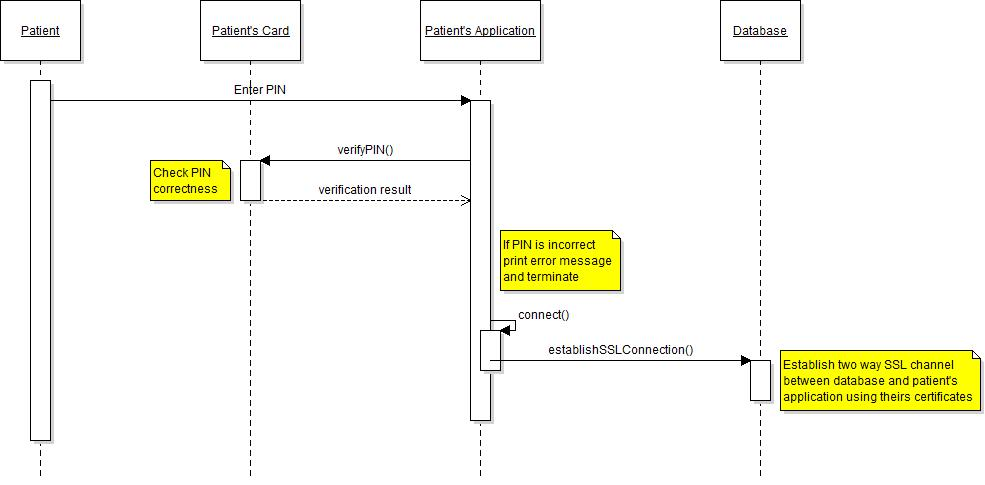
\includegraphics[width=\linewidth]{initializeConnectionSequenceDiagram}
\caption{Connection initialization}	
\end{figure}
When the patient connects to the system, he needs to enter the PIN. 
Then, the PIN is verified by the Patient’s Card. 
If the verification fails, an error message is printed and the connection is terminated. 
Otherwise, the Patient’s Application establishes a two-way SSL channel with the database. 
From this point, the communication between the Patient’s Application and the database is done through SSL encrypted channel.

\FloatBarrier

\newpage
\subsection{\textsc{Sequence diagram for transfer prescription functionality}}
\begin{figure}[!h]
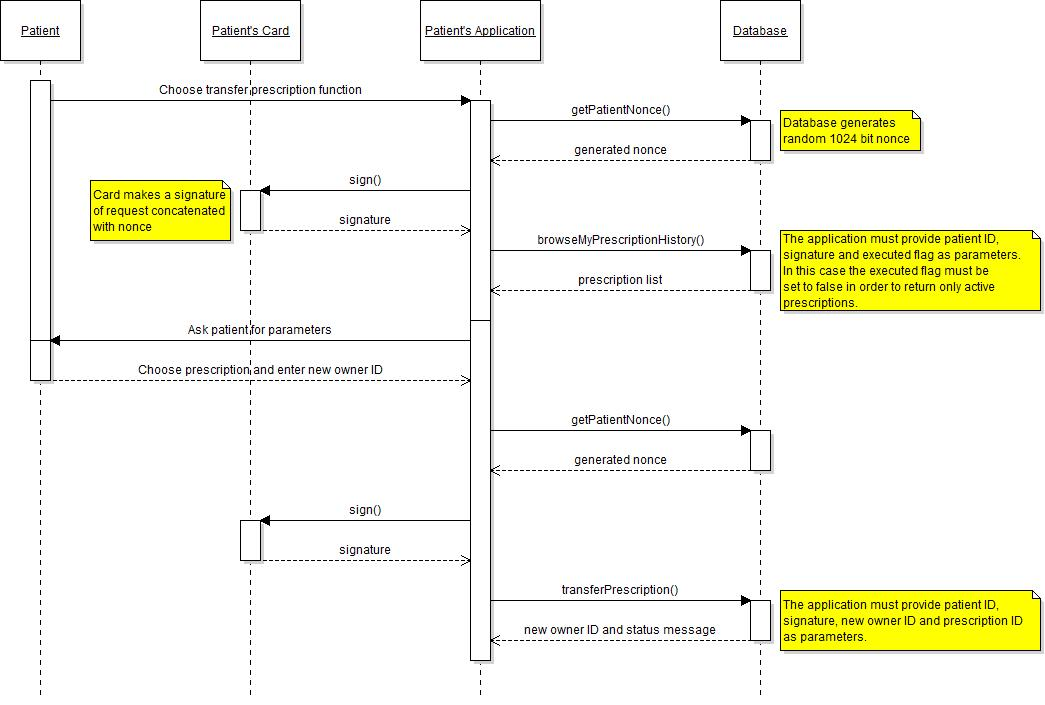
\includegraphics[width=\linewidth]{transferPrescriptionSequenceDiagram}
\caption{Transfer prescription}
\end{figure}
This sequence is executed after establishing a secure connection with the database.\\

To transfer a prescription, the patient has to choose transfer prescription functionality in the Patient’s Application (PA). 
PA sends patient’s ID to the database and receives a random 1024 bit nonce. 
Afterwards, PA sends created browse prescriptions request to the Patient’s Card (PC) for signing. 
PA sends the signed request to the database (DB) and receives a list of available prescriptions. 
Then the patient chooses a prescription he wants to transfer from the list, and enters new owner’s ID.
Next, PA requests new nonce from DB and creates a valid transfer prescription request, which is signed by PC. 
The request with a signature is sent to DB afterwards. 
DB verifies both the request and the signature. If the verification was successful, DB transfers the prescription to the new owner and returns a status message and the ID of new owner.
\FloatBarrier

\newpage
\subsection{\textsc{Sequence diagram for browse medicines functionality}}
\begin{figure}[!h]
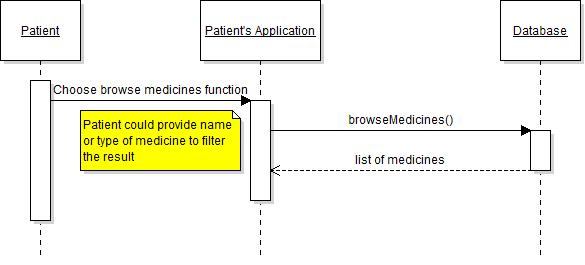
\includegraphics[width=\linewidth]{browseMedicinesSequenceDiagram}
\caption{Browse medicines}
\end{figure}
To browse medicines, the patient needs to choose browse medicines functionality in the Patient’s Application. 
Then, the Patient’s Application prepares a request with parameters either default or provided by the patient. 
The request is sent to the database afterwards. 
The database returns a list of medicines which is displayed to the patient in the Patient’s Application.
\newpage


\section{\textsc{Security}}

Both security mechanisms used in the patient's module and their justification are described in the following sections.

\subsection{\textsc{Used security mechanisms}}

\subsubsection{\textsc{Smart card}}

\begin{tabularx}{\textwidth}{ |p{2.5cm}|X| }
	\hline
	\textbf{Entity} &  \textbf{Description}\\
	\hline	
Patient's card & Patient's card stores private key along with the certificate. Elements of the certificate are as follows (text in parentheses describes what is used): 
\begin{itemize}
\item Serial Number: Used to uniquely identify the certificate
\item Subject: The person, or entity identified (personal data of the patient).
\item Signature Algorithm: The algorithm used to create the signature (RSA).
\item Signature: The actual signature to verify that it came from the issuer.
\item Issuer: The entity that verified the information and issued the certificate (CA for the patient).
\item Valid-From: The date the certificate is first valid from.
\item Valid-To: The expiration date.
\item Public Key: The public key.
\item Thumbprint Algorithm: The algorithm used to hash the public key certificate (SHA256).
\item Thumbprint (also known as fingerprint): The hash itself, used as an abbreviated form of the public key certificate.
\end{itemize} \\
\hline
	
Card's data \newline access &
\begin{itemize}
\item 
Card is read only is the sense that patients are not able to modify the data that is stored on it. They do, however (after successful authentication), have access to certificate stored on the card as well as the function to sign arbitrary input data with its private key.
\end{itemize} \\
\hline

PIN &
\begin{itemize}
\item The certificate access/signing input data can be performed after entering PIN. The user is given 4-digit PIN and the verification system will allow three attempts before blocking the card.
\end{itemize} \\
\hline
\end{tabularx}

\subsubsection{\textsc{Authentication}}

Patient's authentication is constructed as a two factor process. It includes the following points:
\begin{itemize}
\item Something you have - smart card (containing user's certificate)
\item Something you know - PIN needed to access smart card's functionalities
\end{itemize}

\subsubsection{\textsc{Connection}}

The connection between the application and the database is established by two-way SSL protocol. Whole communication afterwards would be sent by encrypted SSL channel. We assume that if the connection was lost, the whole authentication process needs to be repeated.

\subsection{\textsc{Justification}}

\subsubsection{\textsc{PIN protection}}

The PIN number is used to authenticate the cardholder. We propose 4-digit PIN number. Three subsequent incorrect attempts will block the card. Similar mechanism is already used e.g. in ATM cards.	

\subsubsection{\textsc{Secure communication with the database}}

The communication channel between the database and the application is secured with a two way SSL protocol. We assume that SSL provides all necessary mechanisms to protect the channel from attacks.

\subsubsection{\textsc{Protection against prescription overtaking}}

Transfer prescription request have to be signed by the patient using his private key in order to not give buying rights to unauthorized person. If the patient has made a mistake during prescription transfer, he is able to cancel and redo the transfer correctly.

\subsubsection{\textsc{Protection against prescription duplication}}

Transfer and cancel transfer prescription functionalities have to be performed in transaction environment by the database. In this way, there would be no possibility that both the patient and new owner could buy the prescription simultaneously.


\subsection{Advantages of system}

Our system is designed in way that any defraudation of purchasing not prescribed medicine is impossible, pharmacist can not do any defraudation on transaction of seeling drugs to the patient which were not previously prescribed by the doctor, because to every transaction our system demands patient's smart card with previously issued prescription by the doctor and signed by his smart card.
\\

The above security assure very secure system of digital signatures and certificates which will be implemented in our application on smart cards and users programs. This system will prevent any defraudation from users (patient/ pharmacist/ doctor) and also simplify any financial settlement between pharmacist and NFZ, furthermore system will be very comfortable and easy to use for every user.
\end{document}

